\documentclass[12pt, a4paper, oneside]{ctexart}
\usepackage{amsmath, amsthm, amssymb, bm, color, enumerate, framed, graphicx, longtable, mathrsfs, subfigure, tikz}
\usepackage{geometry}
\geometry{left=2.54cm,right=2.54cm,top=3.18cm,bottom=3.18cm}

% 超链接设置
\usepackage{hyperref}
\hypersetup{  
    colorlinks = true,    % 更改链接颜色  
    linkcolor = blue,      % 链接颜色  
    urlcolor = blue,        % URL 颜色  
    citecolor = green,     % 引用颜色  
    % underline = true,  
    linkbordercolor = red,
}
% \hypersetup{colorlinks=true,linkcolor=black}

%代码包设置
\usepackage{listings}
\lstset{
    basicstyle          =   \sffamily,          % 基本代码风格
    keywordstyle        =   \bfseries,          % 关键字风格
    commentstyle        =   \rmfamily\itshape,  % 注释的风格,斜体
    stringstyle         =   \ttfamily,  % 字符串风格
    flexiblecolumns,                % 别问为什么,加上这个
    numbers             =   left,   % 行号的位置在左边
    showspaces          =   false,  % 是否显示空格,显示了有点乱,所以不现实了
    numberstyle         =   \zihao{-5}\ttfamily,    % 行号的样式,小五号,tt等宽字体
    showstringspaces    =   false,
    captionpos          =   t,      % 这段代码的名字所呈现的位置,t指的是top上面
    frame               =   lrtb,   % 显示边框
}
\lstdefinestyle{C}{
    language        =   C, % 语言选C
    basicstyle      =   \zihao{-5}\ttfamily,
    numberstyle     =   \zihao{-5}\ttfamily,
    keywordstyle    =   \color{blue},
    keywordstyle    =   [2] \color{teal},
    stringstyle     =   \color{magenta},
    commentstyle    =   \color{red}\ttfamily,
    breaklines      =   true,   % 自动换行,建议不要写太长的行
    columns         =   fixed,  % 如果不加这一句,字间距就不固定,很丑,必须加
    basewidth       =   0.5em,
}

% 设置思源宋体为中文字体
\setCJKsansfont{Source Han Serif SC}

% 设置思源黑体为中文字体
\setCJKsansfont{Source Han Sans SC}

% 设置arev为英文字体
\setsansfont{Arev Sans}

% 字体颜色
\def\red{\color{red}}
\def\blue{\color{blue}}
\def\black{\color{black}}
\def\green{\color{green}}

\title{\textbf{操作系统课程作业}}
\author{162140222黄钰轩}
\date{\today}
\linespread{1.25}

\definecolor{shadecolor}{RGB}{241, 241, 255}
\newcounter{problemname}
\newenvironment{problem}{\begin{shaded}\stepcounter{problemname}\par\noindent\textbf{题目\arabic{problemname}. }}{\end{shaded}\par}
\newenvironment{solution}{\par\noindent\textbf{解答. }}{\par}
\newenvironment{note}{\par\noindent\textbf{题目\arabic{problemname}的注记. }}{\par}
%\renewcommand{\proofname}{\bf 证明}

\begin{document}

\begin{figure}[t]
    \centering
    
\includegraphics[width=13cm]{images/logo.png}
\end{figure}

\maketitle

\begin{problem}
    一般操作系统中,进程的每个段内部地址均连续,但段与段的相对次序可能不同,请你用 C/CPP 语言写一个探测程序,探测 Windows、Linux 操作系统中进程的各段的相对位置(输出次序即可).
\end{problem}

\begin{solution}
    具体实现思路请查看 \href{run:./README.md}{README.md},程序代码如下:
    \lstinputlisting[
        style       =   C,
        caption     =   {\bf probe.c},
        label       =   {probe.c}
    ]{./probe.c}
    这里使用了条件编译,判断宏 \_WIN32 是否有定义,即可分别在不同的操作系统中进行验证. 当进入 Linux 系统时,保持代码不变,而当进入 Windows 系统时,只需将第三行注释掉,即可正常编译.
    \newpage
    经测试,在两个系统中分别编译的结果如下:
    \begin{figure}[!htbp]
        \centering
        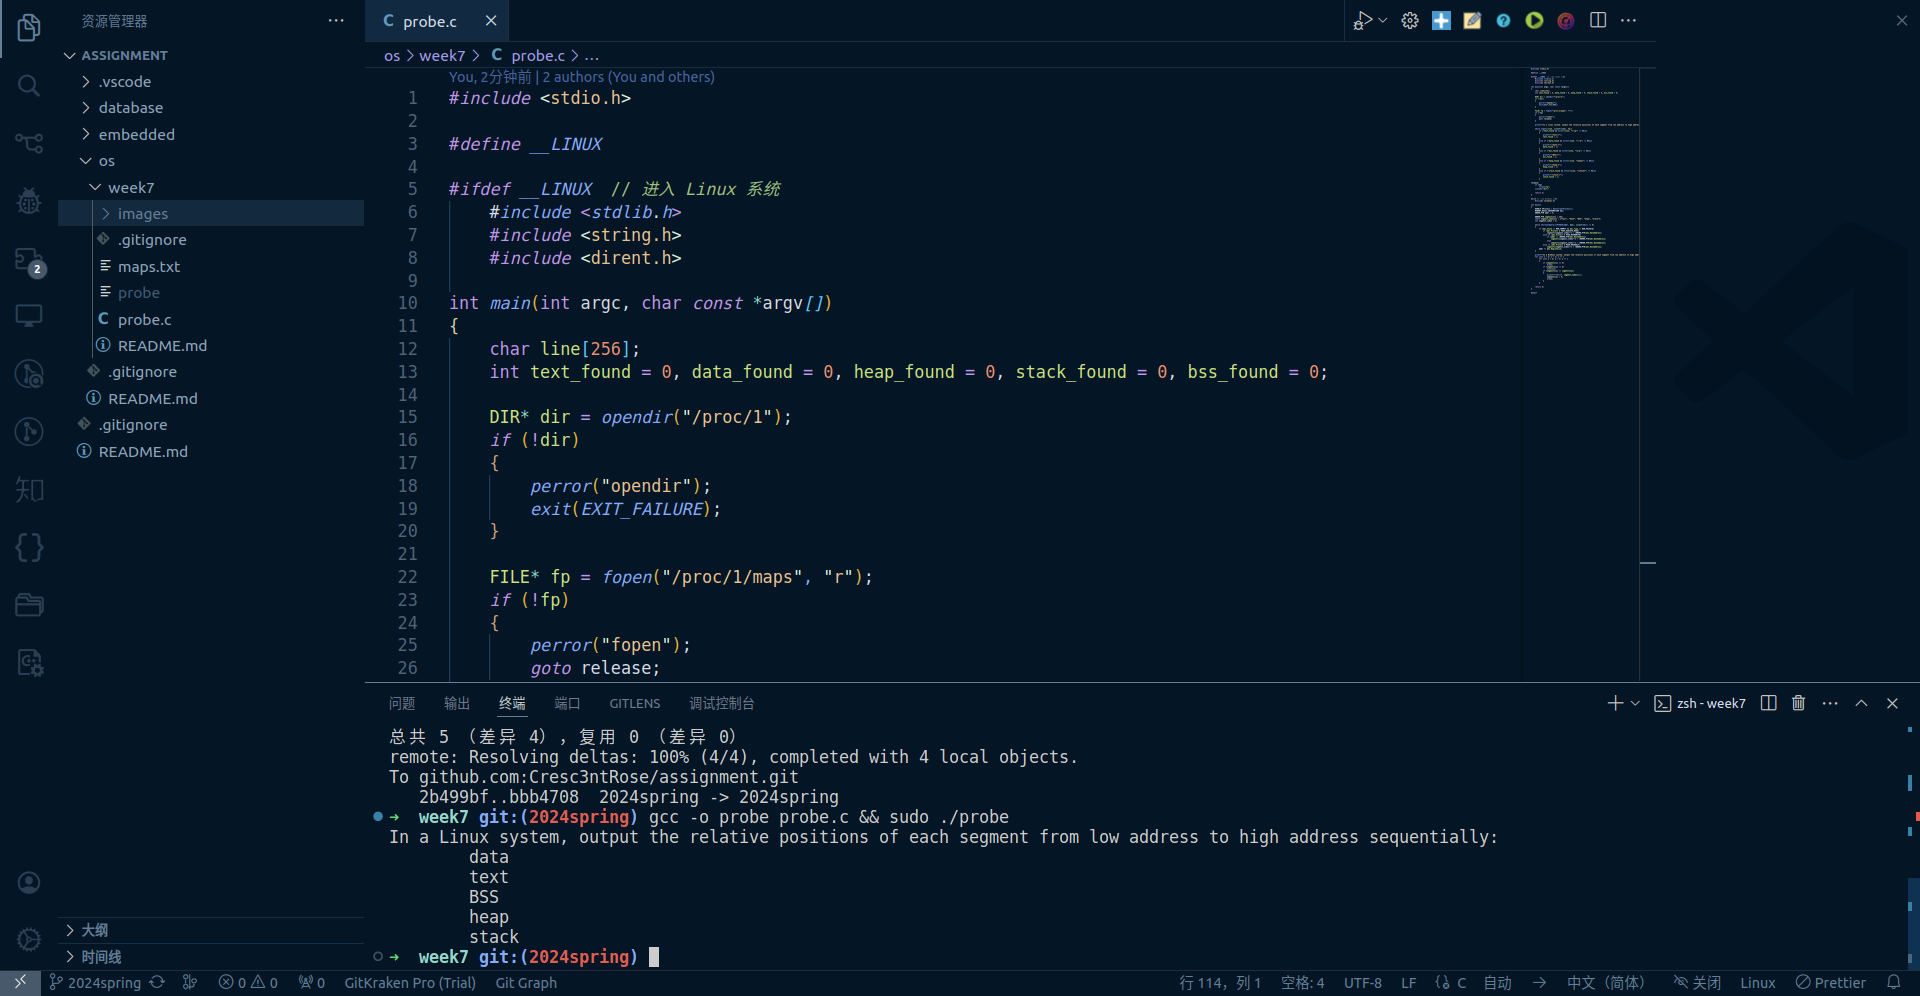
\includegraphics[width=13cm]{images/Probe_Linux.png}
        \caption{Linux 系统下编译代码}
    \end{figure}
    \begin{figure}[!htbp]
        \centering
        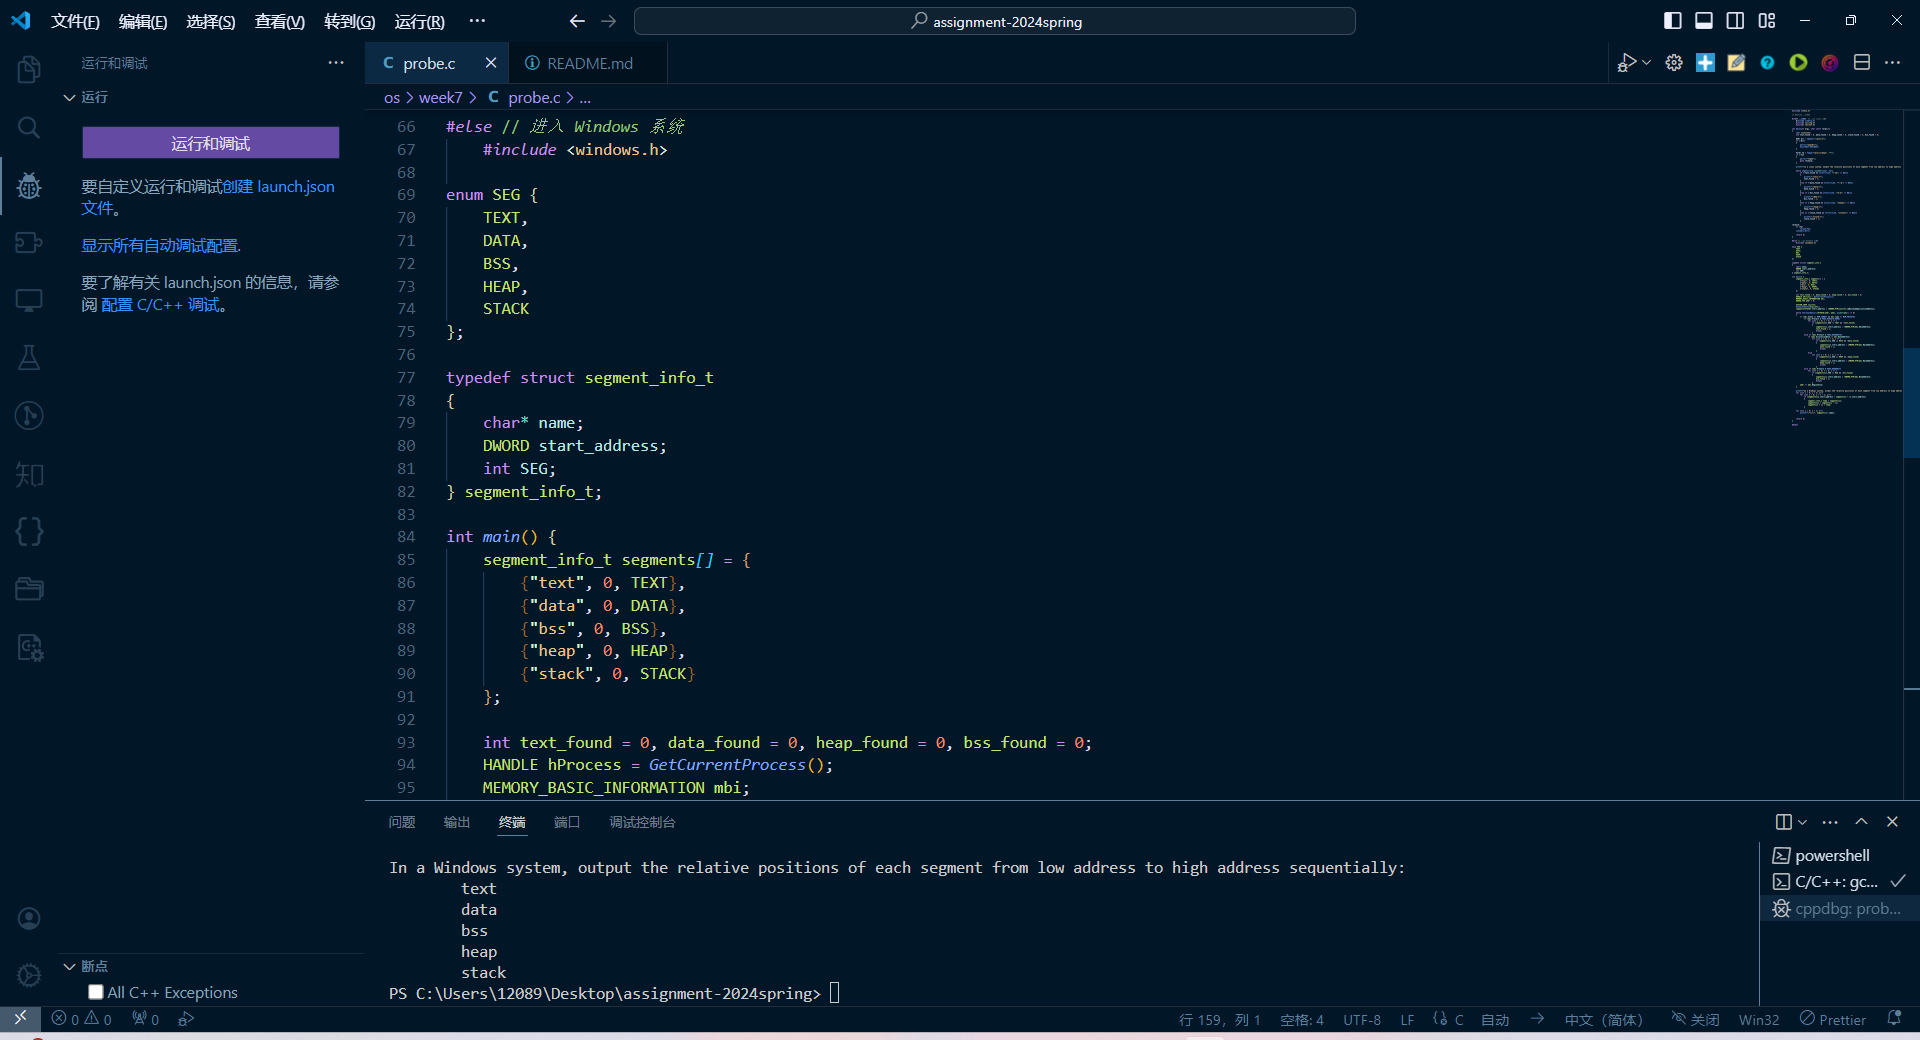
\includegraphics[width=13cm]{images/Probe_Windows.png}
        \caption{Windows 系统下编译代码}
    \end{figure}
\end{solution}

\begin{note}
    Linux 提供了 \href{https://en.wikipedia.org/wiki/Procfs}{procfs},目录是 /proc,而 /proc/[pid]/\href{run:./images/maps.png}{maps} 文件中就蕴含着完成这个作业所需的全部信息.
\end{note}

\begin{problem}
    实现一程序,分别在 Windows、Linux 操作系统下验证:
    \begin{enumerate}[(1)]
        \item 栈、堆、数据区是否可读可写不可执行.
        \item 代码段是否可读不可写可执行.
    \end{enumerate}
\end{problem}

\begin{solution}
    具体实现思路请查看 \href{run:./README.md}{README.md}. 在 Windows 系统下,我选择使用C语言进行验证:
    \lstinputlisting[
        style       =   C,
        caption     =   {\bf checker.c},
        label       =   {checker.c}
    ]{./checker.c}
    在 Windows 系统中编译结果如下:
    \begin{figure}[!htbp]
        \centering
        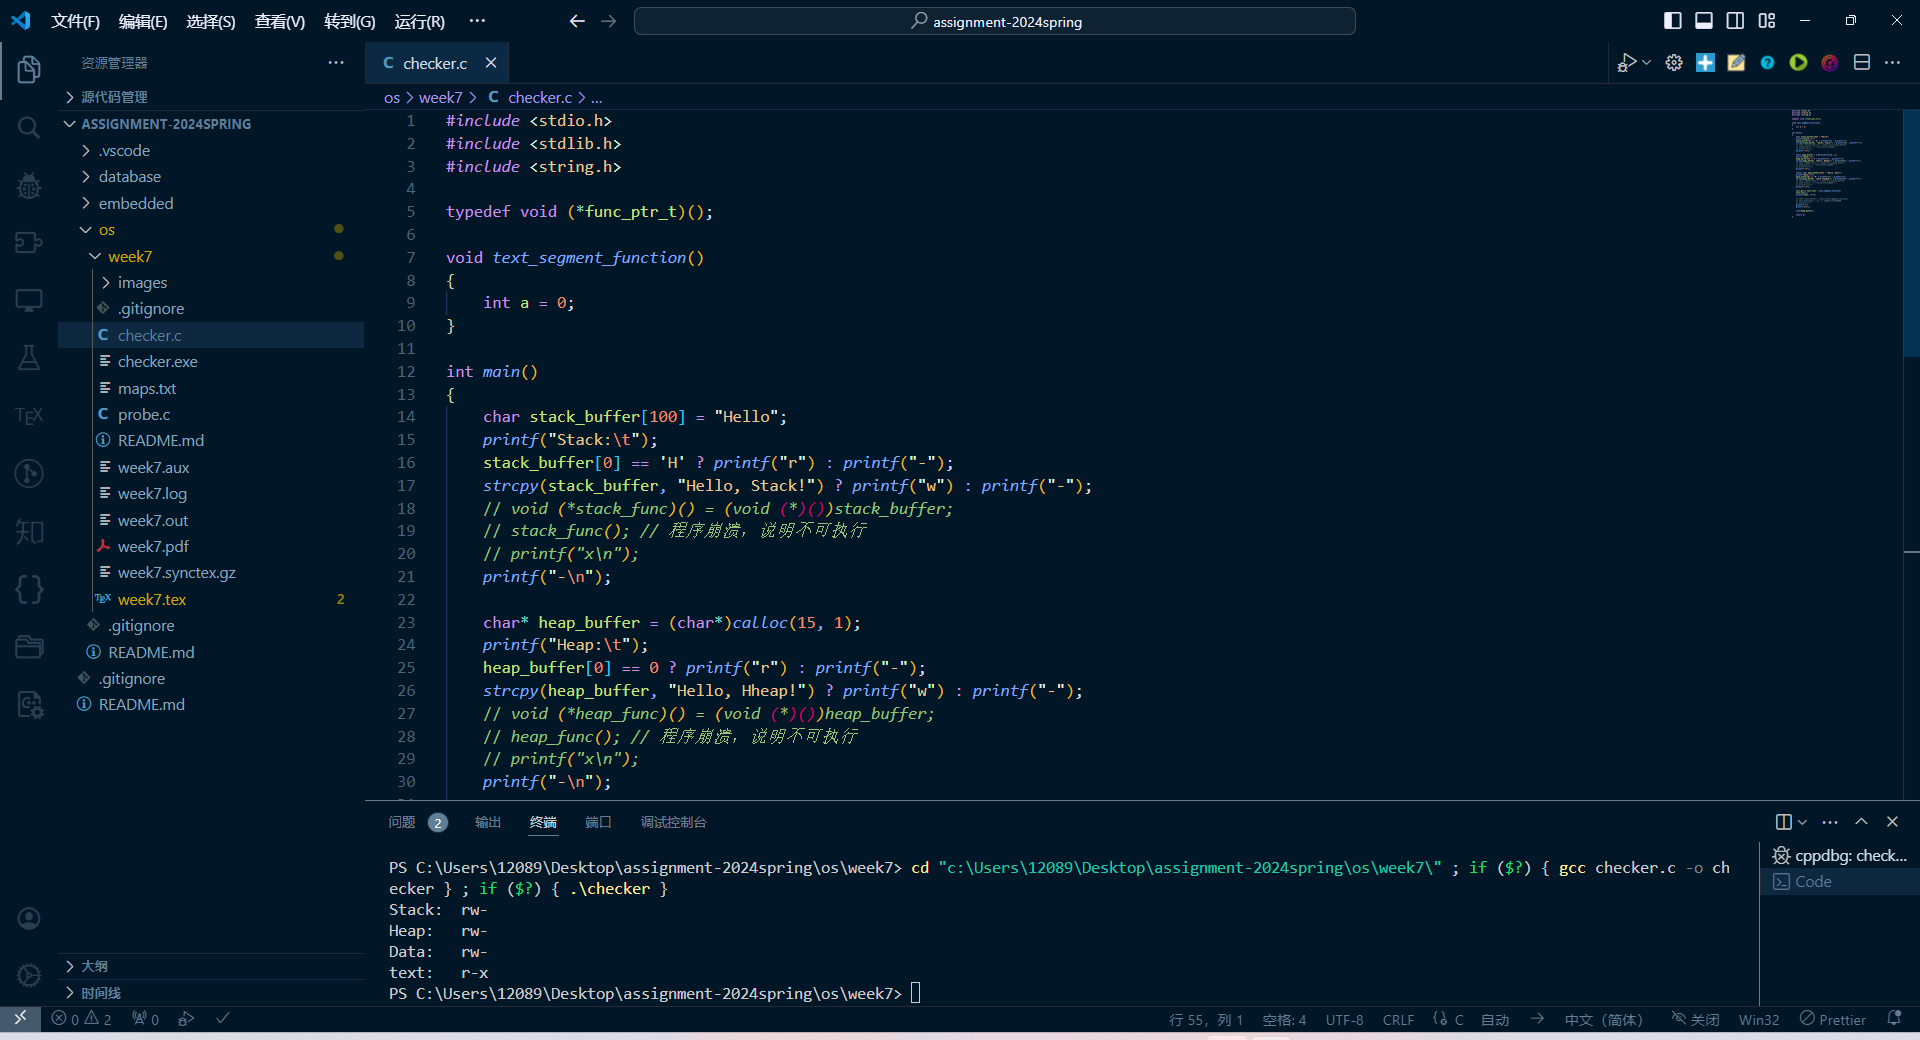
\includegraphics[width=12cm]{images/Checker_Windows.png}
        \caption{Windows 系统下编译代码}
    \end{figure}
    \newline
    如果将代码中被注释的部分取消注释,那么就会引发程序崩溃.
    \begin{figure}[!htbp]
        \centering
        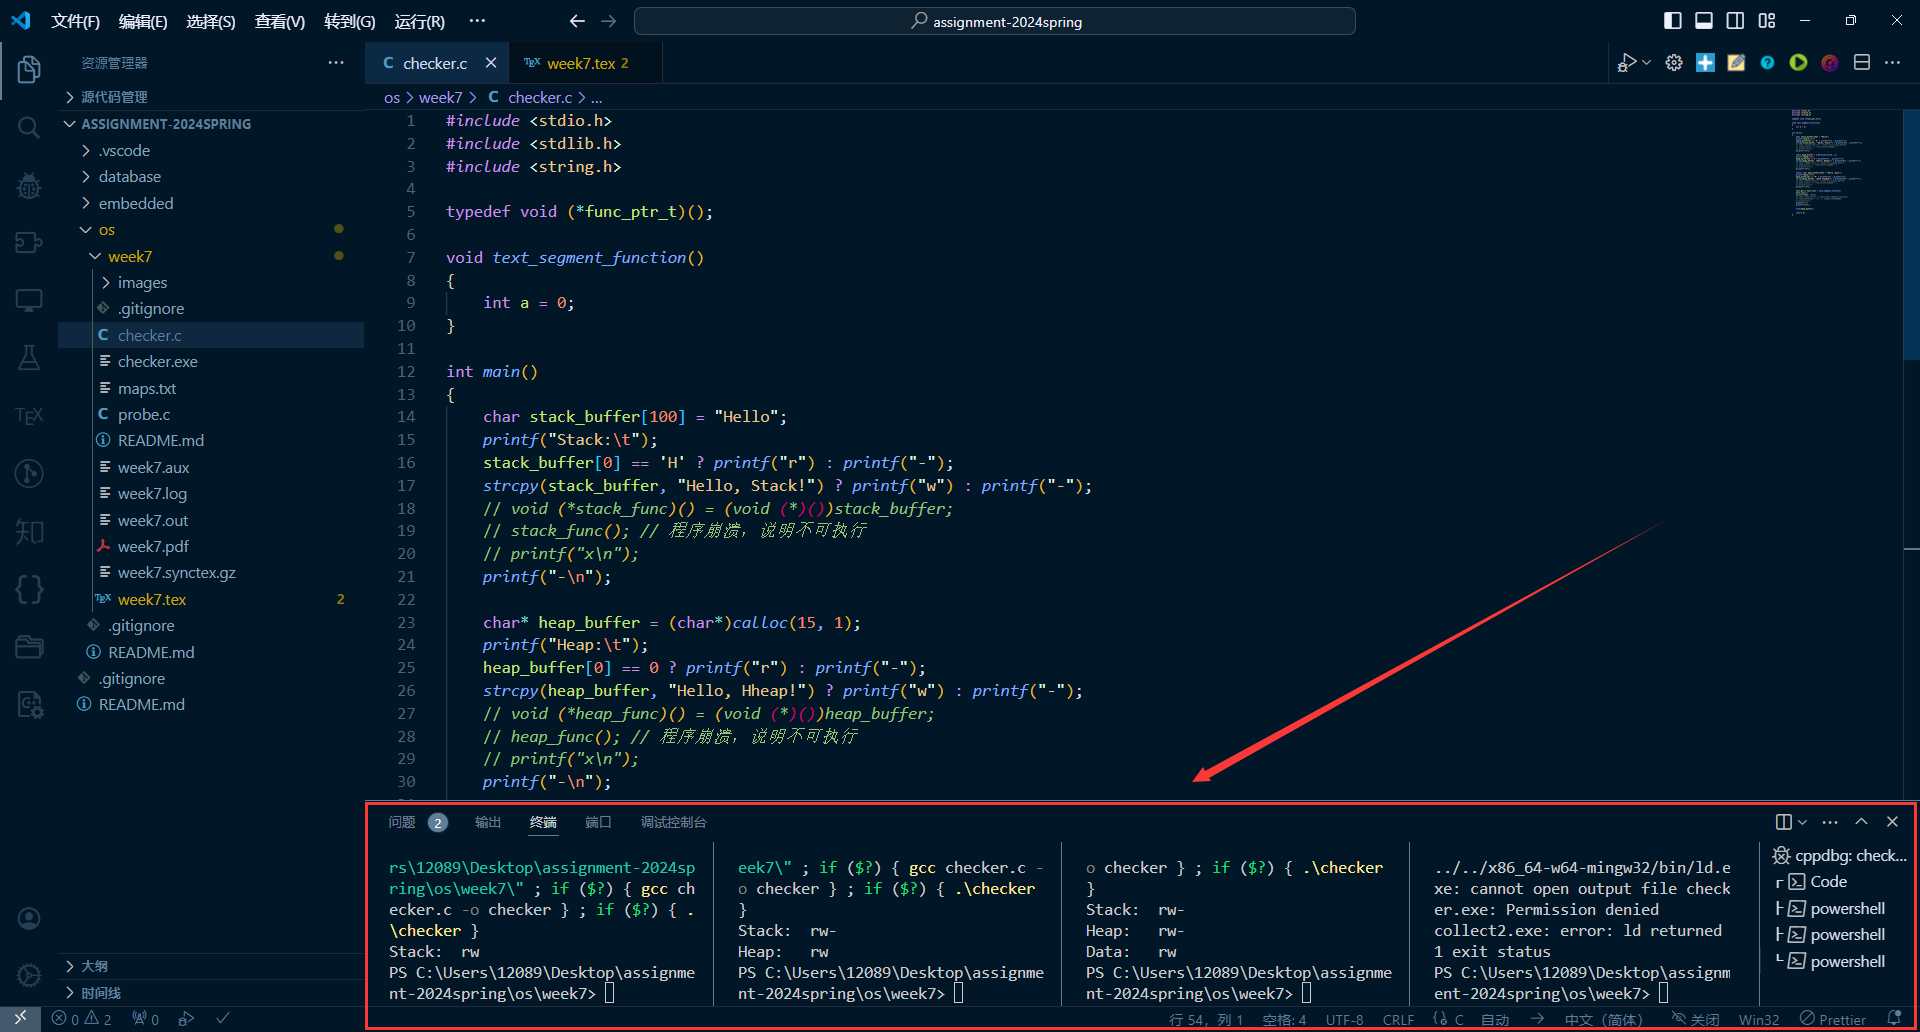
\includegraphics[width=13cm]{images/Checker_Windows_Error.png}
        \caption{Windows 系统下编译代码}
    \end{figure}
    \newpage
    该程序在 Linux 系统下一样可以得到验证:
    \begin{figure}[!htbp]
        \centering
        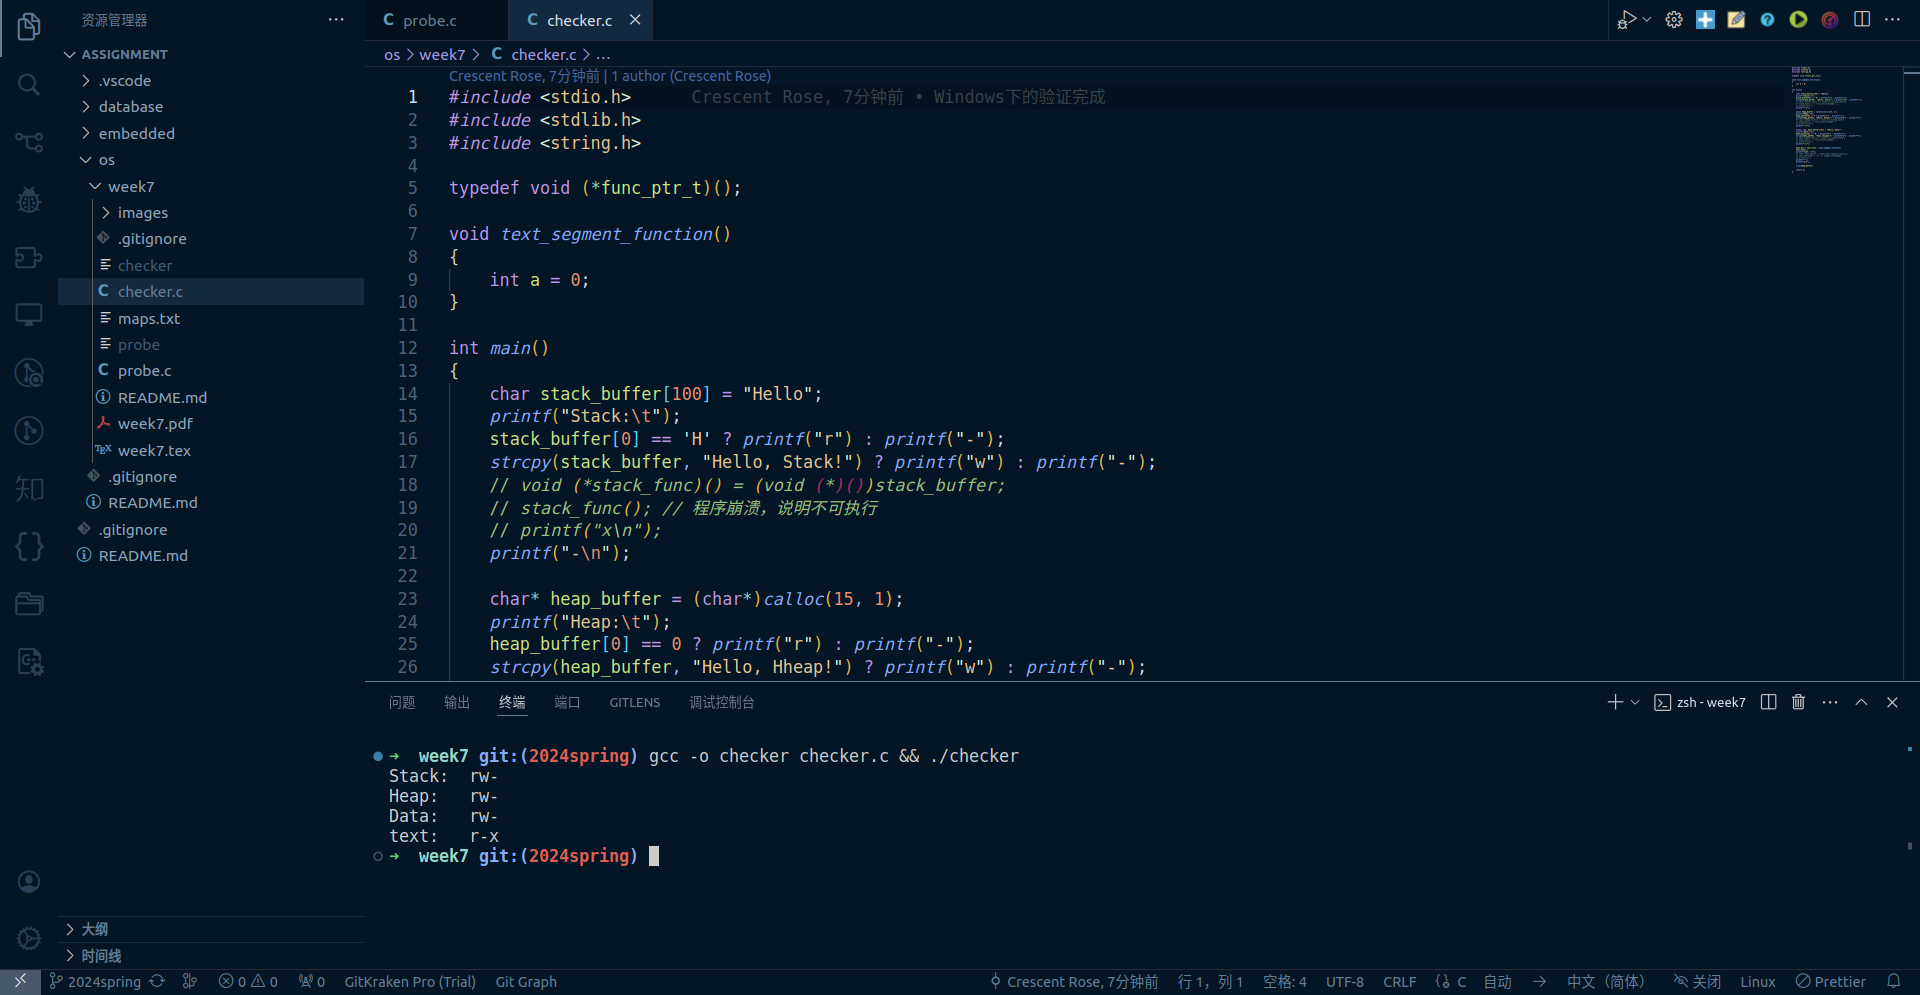
\includegraphics[width=13cm]{./images/Checker_Linux.png}
        \caption{Windows 系统下编译代码}
    \end{figure}\newline
    同时,在 Linux 系统下,我尝试了使用 rust 语言构建程序进行验证:
    \begin{figure}[!htbp]
        \centering
        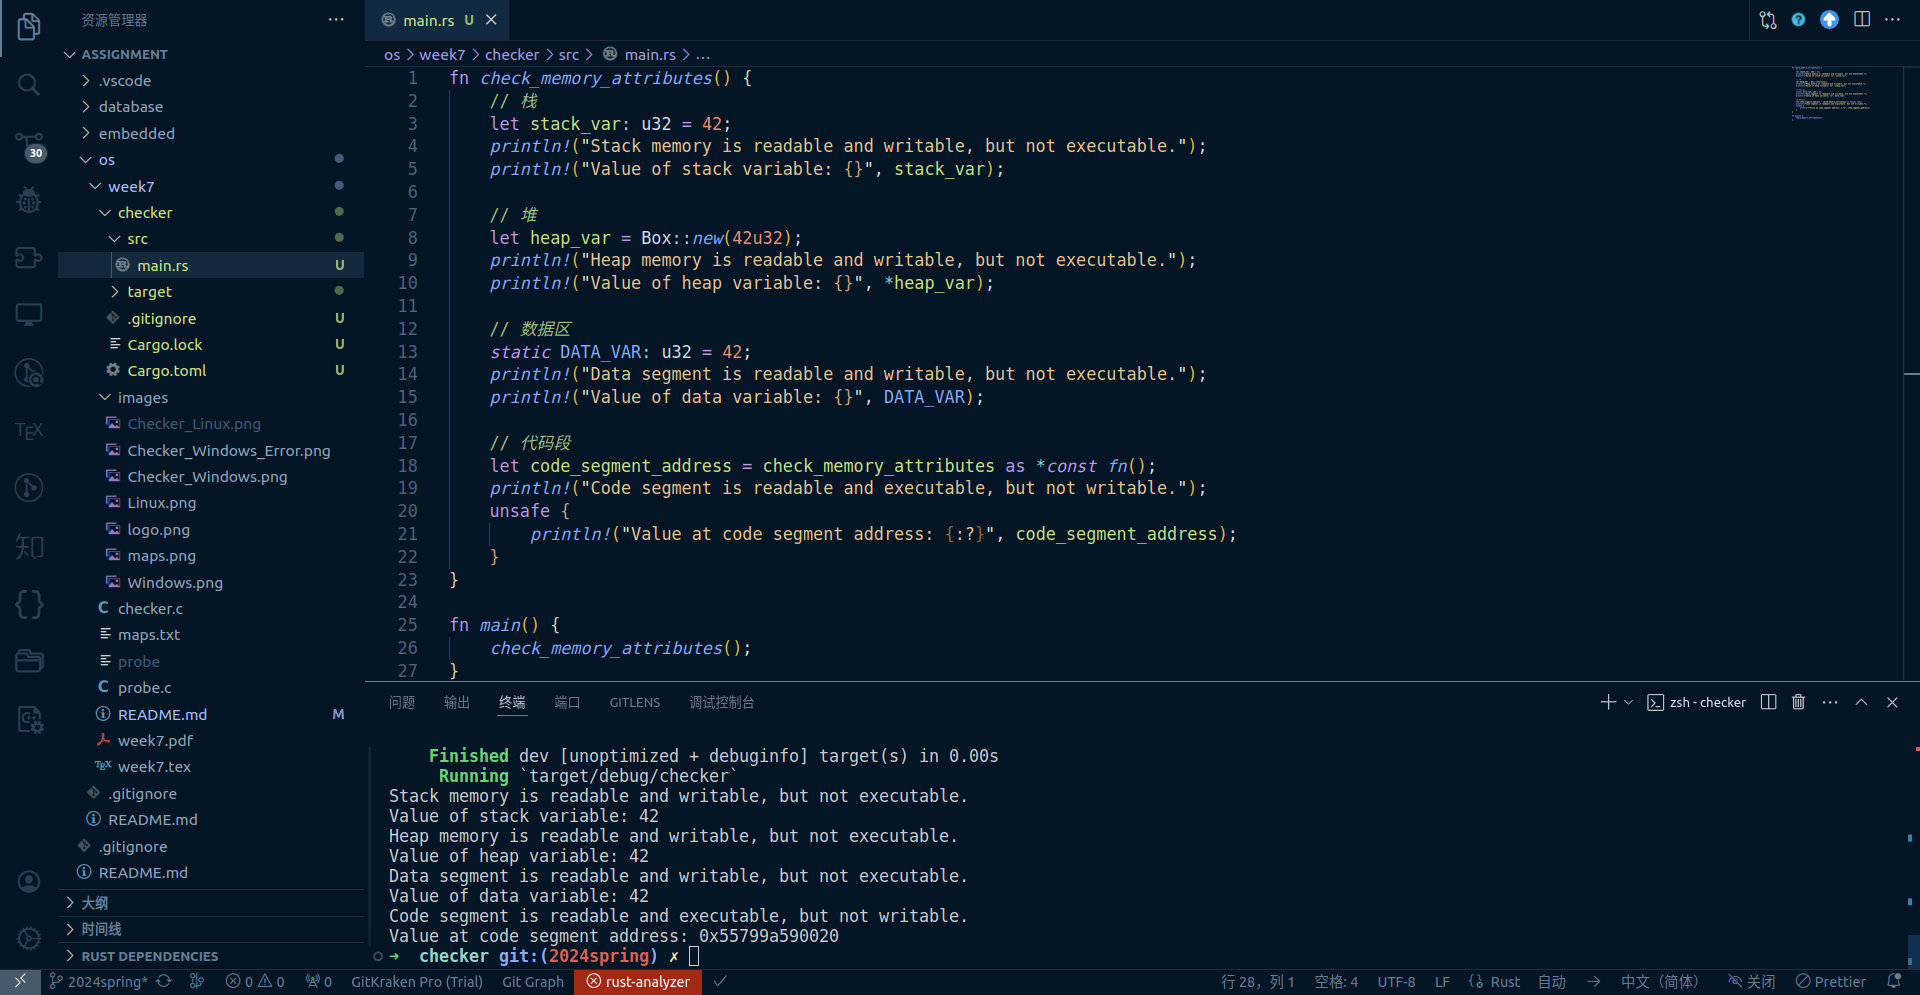
\includegraphics[width=13cm]{./images/Checker_Rust.png}
        \caption{Windows 系统下编译代码}
    \end{figure}\newline
    最终同样完成了验证.
\end{solution}

\end{document}